\documentclass[tikz,border=5]{standalone}
\usepackage{tikz, pgfplots}

\usetikzlibrary{arrows.meta}
\usetikzlibrary{shapes,arrows}
\usetikzlibrary{calc}
\usetikzlibrary{patterns}
\usetikzlibrary{fit}

\tikzstyle{decision} = [diamond, draw, fill=blue!20,
    text width=4.5em, text badly centered, node distance=3cm, inner sep=0pt]
\tikzstyle{block} = [rectangle, draw, fill=blue!20,
    text width=7em, text centered, rounded corners, minimum height=3em]
\tikzstyle{line} = [draw, -latex']
\tikzstyle{cloud} = [draw, ellipse,fill=red!20, node distance=3cm,
    minimum height=3em, minimum width=7em]


\begin{document}


\begin{tikzpicture}[node distance = 2cm, scale=0.8]
%    \node [cloud] (atom) {ASE-Atom Class};
	\node at (0,1) [cloud] (atoms) {ASE.Atoms};
	\node at (6,1) [cloud] (list) {List};
%	\node [cloud, right of=atom, node distance = 4cm] (O1) {Atom};
	\node at (0,-1.5) [cloud] (O2) {System};
	\node at (6, -1.5) [cloud] (O8) {Trajectory};
	\node at (-3.5,-4.5) [block] (O3) {Solid State \\ 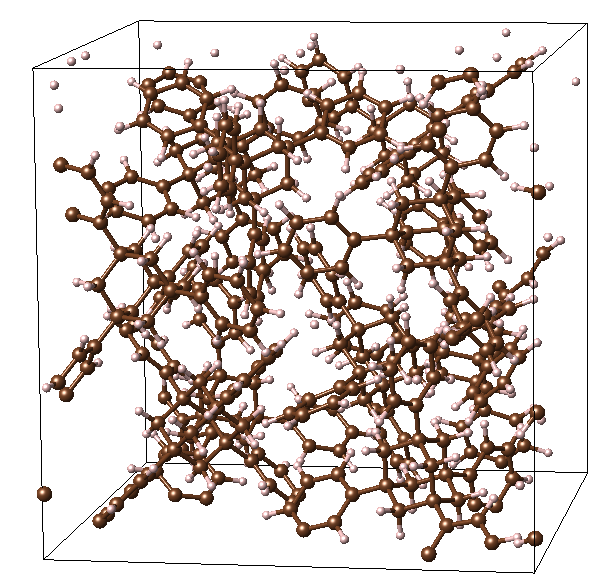
\includegraphics[width=0.5\textwidth]{images/solid.png}};
	\node at (3.5,-4.5) [block] (O4) {Dimer \\ 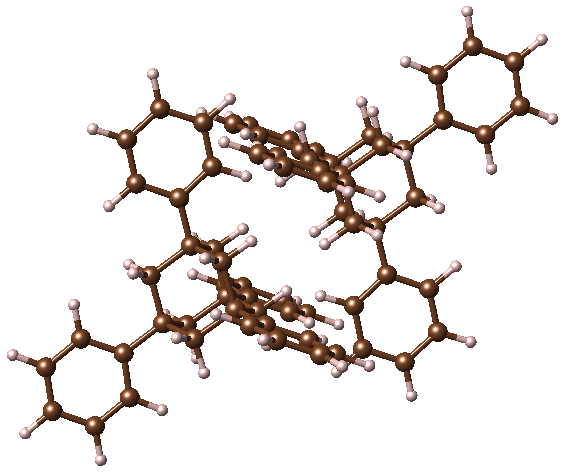
\includegraphics[width=0.5\textwidth]{images/dimer.png}};
	\node at (0,-7.5) [block] (O5) {Molecule \\ 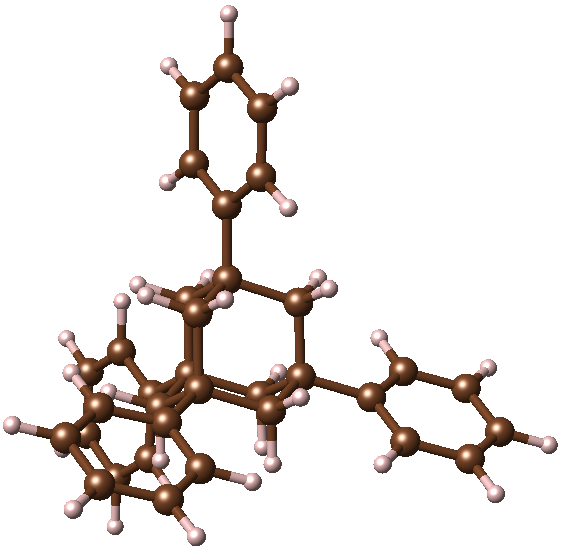
\includegraphics[width=0.5\textwidth]{images/mono.png}};
	\node at (-3.5,-10.5) [block] (O6) {Core \\ 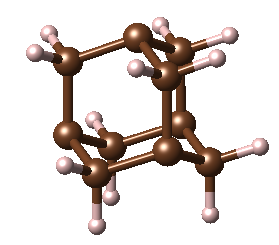
\includegraphics[width=0.5\textwidth]{images/core.png}};
	\node at (3.5, -10.5) [block] (O7) {Substituent \\
	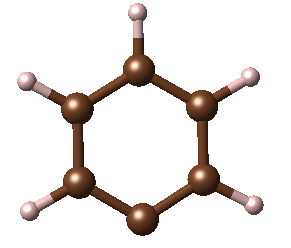
\includegraphics[width=0.5\textwidth]{images/substituent.png}};
%
%	\node [block, right of=O3, node distance = 3.5cm] (D3) {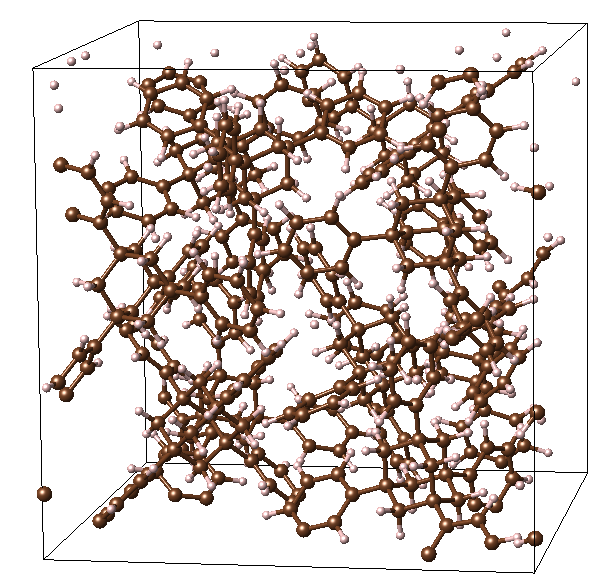
\includegraphics[width=.7\textwidth]{images/solid.png}};
%	\node [block, right of=O4, node distance = 3.5cm] (D4) {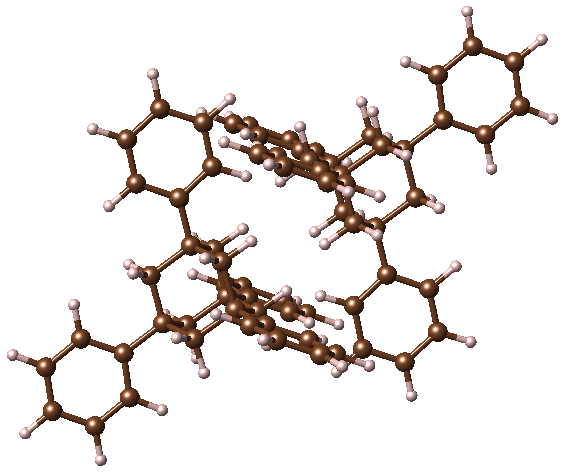
\includegraphics[width=.7\textwidth]{images/dimer.png}};
%	\node [block, right of=O5, node distance = 3.5cm] (D5) {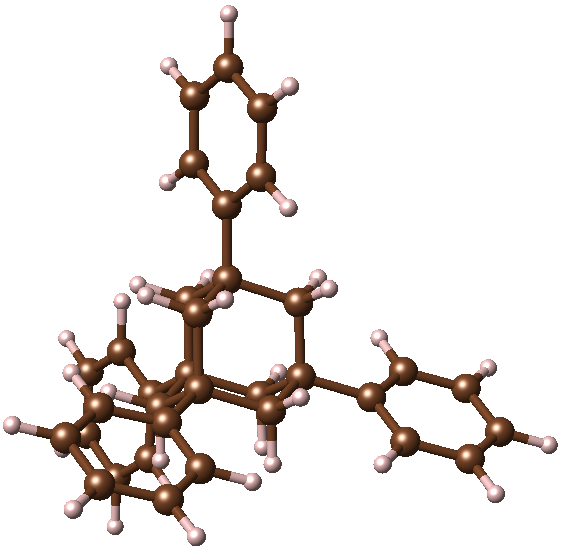
\includegraphics[width=.7\textwidth]{images/mono.png}};
%	\node [block, right of=O6, node distance = 3.5cm] (D6) {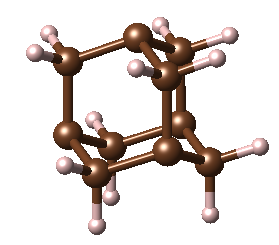
\includegraphics[width=.7\textwidth]{images/core.png}};
%	\node [block, right of=O7, node distance = 3.5cm] (D7) {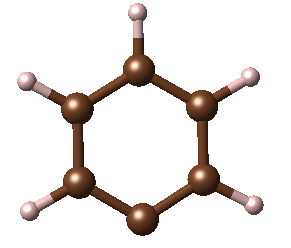
\includegraphics[width=.7\textwidth]{images/substituent.png}};
%
%
    \path [line, dotted] (list) -- (O8);
    \path [line, dotted] (atoms) -- (O2);
    \path [line, dotted] (O2) -- (O3);
    \path [line, dotted] (O2) -- (O4);
    \path [line, dotted] (O2) -- (O5);
	\path [line, dotted] (O2) -- (O6);
    \path [line, dotted] (O2) -- (O7);

	\path [line] (O3) -- (O5);
	\path [line] (O4) -- (O5);

	\path [line] (O5) -- (O6);
	\path [line] (O5) -- (O7);

	\path [line] (O8) -- (O3);
	\path [line] (O8) -- (O4);

%    \path [line, dotted] (O3) -- (D3);
%    \path [line, dotted] (O4) -- (D4);
%    \path [line, dotted] (O5) -- (D5);
%    \path [line, dotted] (O6) -- (D6);
%	\path [line, dotted] (O7) -- (D7);
%
%    \path [line] (D3) -- (O5);
%    \path [line] (D4) -- (O5);
%    \path [line] (D5) -- (O6);
%    \path [line] (D5) -- (O7);
%	\path [line] (O8) -- (O3);
%    \path [line] (O8) -- (O4);


\end{tikzpicture}

\end{document}

